%%%%%%%%%%%%%%%%%%%%%%%%%%%%%%%%%%%%%%%%%
% Beamer Presentation
% LaTeX Template
% Version 1.0 (10/11/12)
%
% This template has been downloaded from:
% http://www.LaTeXTemplates.com
%
% License:
% CC BY-NC-SA 3.0 (http://creativecommons.org/licenses/by-nc-sa/3.0/)
%
%%%%%%%%%%%%%%%%%%%%%%%%%%%%%%%%%%%%%%%%%

%----------------------------------------------------------------------------------------
%	PACKAGES AND THEMES
%----------------------------------------------------------------------------------------

\documentclass{beamer}

\mode<presentation> {

% The Beamer class comes with a number of default slide themes
% which change the colors and layouts of slides. Below this is a list
% of all the themes, uncomment each in turn to see what they look like.

%\usetheme{default}
%\usetheme{AnnArbor}
%\usetheme{Antibes}
%\usetheme{Bergen}
%\usetheme{Berkeley}
%\usetheme{Berlin}
%\usetheme{Boadilla}
%\usetheme{CambridgeUS}
%\usetheme{Copenhagen}
\usetheme{Darmstadt}
%\usetheme{Dresden}
%\usetheme{Frankfurt}
%\usetheme{Goettingen}
%\usetheme{Hannover}
%\usetheme{Ilmenau}
%\usetheme{JuanLesPins}
%\usetheme{Luebeck}
%\usetheme{Madrid}
%*\usetheme{Malmoe}
%\usetheme{Marburg}
%\usetheme{Montpellier}
%\usetheme{PaloAlto}
%\usetheme{Pittsburgh}
%\usetheme{Rochester}
%\usetheme{Singapore}
%\usetheme{Szeged}
%\usetheme{Warsaw}

% As well as themes, the Beamer class has a number of color themes
% for any slide theme. Uncomment each of these in turn to see how it
% changes the colors of your current slide theme.

%\usecolortheme{albatross}
%\usecolortheme{beaver}
%\usecolortheme{beetle}
%\usecolortheme{crane}
%\usecolortheme{dolphin}
%\usecolortheme{dove}
%\usecolortheme{fly}
%\usecolortheme{lily}
\usecolortheme{orchid}
%\usecolortheme{rose}
%\usecolortheme{seagull}
%\usecolortheme{seahorse}
%\usecolortheme{whale}
%\usecolortheme{wolverine}

%\setbeamertemplate{footline} % To remove the footer line in all slides uncomment this line
%\setbeamertemplate{footline}[page number] % To replace the footer line in all slides with a simple slide count uncomment this line

%\setbeamertemplate{navigation symbols}{} % To remove the navigation symbols from the bottom of all slides uncomment this line
}


\usepackage{graphicx} % Allows including images
\usepackage{booktabs} % Allows the use of \toprule, \midrule and \bottomrule in tables
\usepackage{xspace}
\usepackage{caption}
\usepackage{subfigure}
\usepackage[english,brazil]{babel}
\usepackage[utf8]{inputenc}

%Renomeia o nome padrao das figuras.
\renewcommand{\figurename}{Figura}
\renewcommand{\tablename}{Tabela}
%----------------------------------------------------------------------------------------
%	TITLE PAGE
%----------------------------------------------------------------------------------------

\title[Computação Gráfica]{Visualização - 3D} % The short title appears at the bottom of every slide, the full title is only on the title page

\author{Uéliton Freitas} % Your name
\institute[UFMS] % Your institution as it will appear on the bottom of every slide, may be shorthand to save space
{
Universidade Católica Don Bosco - UCDB \\ % Your institution for the title page
\medskip
\textit{freitas.ueliton@gmail.com} % Your email address
}
\date{\today} % Date, can be changed to a custom date


\begin{document}

\begin{frame}
\titlepage % Print the title page as the first slide
\end{frame}

\begin{frame}
\frametitle{Sumário} % Table of contents slide, comment this block out to remove it
\tableofcontents % Throughout your presentation, if you choose to use \section{} and \subsection{} commands, these will automatically be printed on this slide as an overview of your presentation
\end{frame}




%----------------------------------------------------------------------------------------
%	PRESENTATION SLIDES
%----------------------------------------------------------------------------------------

%------------------------------------------------
\section{Introdução} 
%------------------------------------------------

%\section{Speeded-Up Robust Features - SURF} % A subsection can be created just before a set of slides with a common theme to further break down your presentation into chunks
%\section{Baf Of Features and Colors}

%\section{Refer\^encias}
%%%%%%%%%%%%%%%%%%%%%%%%%%%%%%%%%%%%%%%%%%%%%%%%%%%%%%%%%%%%%%%%%%%%%%%%%%%%%%%%%%%%%%%%%%
\begin{frame}
\frametitle{Introdução}


	\begin{block}{Visualização}
		\begin{itemize}
			\item<1-> As funções de visualização processam a descrição dos objetos por meio de vários procedimentos a fim de projetar a visão do objeto na superfície do dispositivo de saída.
			\item<2-> Alguns destes procedimentos são parecidos com com o Pipeline de visualização 2D
				\begin{itemize}
					\item Rotinas de recorte.
				\end{itemize}
			\item Mas há outras rotinas que são específicas do 3D.
			\begin{itemize}
				\item Rotinas de projeção.
				\item Identificação de partes visuais da cena.
				\item Efeitos de Luz.
			\end{itemize}							 		 
		\end{itemize}
	\end{block}
	
\end{frame}



%%%%%%%%%%%%%%%%%%%%%%%%%%%%%%%%%%%%%%%%%%%%%%%%%%%%%%%%%%%%%%%%%%%%%%%%%%%%%%%%%%%%%%%%%%
\begin{frame}
\frametitle{Introdução}


	\begin{block}{Visualização de uma Cena 3D}
		\begin{itemize}
			\item Primeiramente, para obter uma visão de uma cena 3D descritas nas \textbf{coordenadas do mundo}, é necessário definir um sistema de referência para os parâmetros de visão (Câmera).
		
			\begin{itemize}
				\item Definir a posição e orientação do \textbf{plano de visão} ou \textbf{plano de projeção}.
			\end{itemize}
		\end{itemize}
	\end{block}
	
	\begin{figure}[!h]
			\begin{center}
			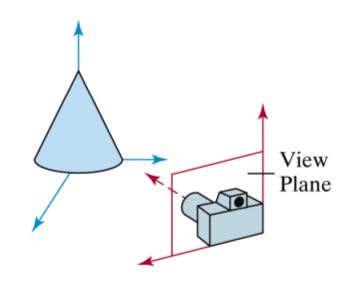
\includegraphics[width=0.5\textwidth]{Figures/ViePla}
			\end{center}
	\end{figure}	
\end{frame}


%%%%%%%%%%%%%%%%%%%%%%%%%%%%%%%%%%%%%%%%%%%%%%%%%%%%%%%%%%%%%%%%%%%%%%%%%%%%%%%%%%%%%%%%%%
\begin{frame}
\frametitle{Introdução}


	\begin{block}{Projeções}
		\begin{itemize}
			\item É possível escolher diferentes métodos para projetar uma cena de visão.
			\begin{itemize}
				\item \textbf{Projeção Paralela} - projeta objetos ao longo de linhas paralelas (Usado para desenhos arquitetônicos).
				\item \textbf{Projeção de Perspectiva} - projeta os pontos de um objeto ao longo de caminhos convergentes produzindo cenas mais realísticas (objetos longe do observador ficam menores).
			\end{itemize}
		\end{itemize}
	\end{block}
	
	\begin{figure}[!h]
			\begin{center}
			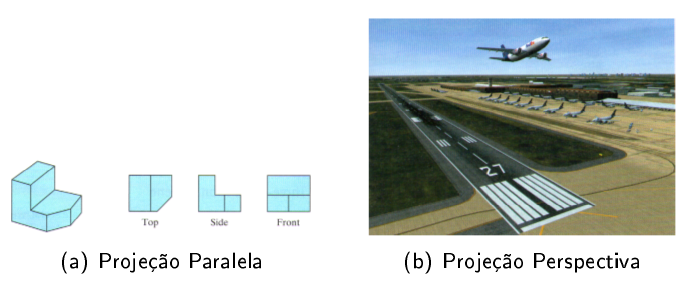
\includegraphics[width=0.5\textwidth]{Figures/Pro}
			\end{center}
	\end{figure}	
\end{frame}

%%%%%%%%%%%%%%%%%%%%%%%%%%%%%%%%%%%%%%%%%%%%%%%%%%%%%%%%%%%%%%%%%%%%%%%%%%%%%%%%%%%%%%%%%%
\begin{frame}
\frametitle{Introdução}


	\begin{block}{Profundidade}
		\begin{itemize}
			\item São raras as exceções em que a profundidade não é importante para composição de uma cena 3D.
			\item A profundidade explicita frente e trás do objeto.
		\end{itemize}
	\end{block}
	
	\begin{figure}[!h]
			\begin{center}
			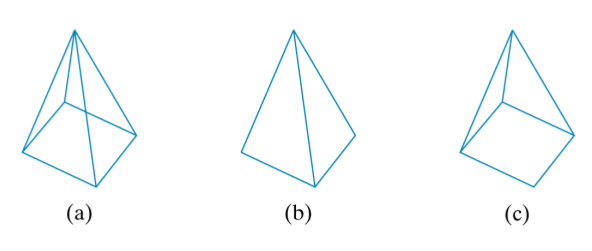
\includegraphics[width=0.5\textwidth]{Figures/ProObj}
			\caption{A Figura a possui problemas de visualização devido a falta de informação de profundidade}
			\end{center}
	\end{figure}	
\end{frame}


%%%%%%%%%%%%%%%%%%%%%%%%%%%%%%%%%%%%%%%%%%%%%%%%%%%%%%%%%%%%%%%%%%%%%%%%%%%%%%%%%%%%%%%%%%
\begin{frame}
\frametitle{Introdução}


	\begin{block}{Identificando Linhas e Superfícies Visíveis}
		\begin{itemize}
			\item Uma forma simples de resolver o problema de profundidade é de objetos aramados (wire-frames) é variar o brilho das linhas.
			\begin{itemize}
				\item Linhas mais próximas da posição de visão possuem maior brilho.
			\end{itemize}
		\end{itemize}
	\end{block}
	
	\begin{figure}[!h]
			\begin{center}
			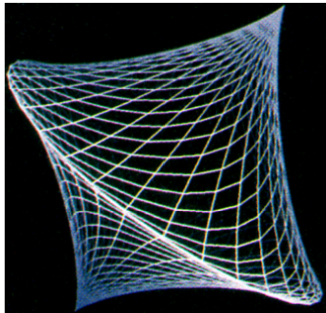
\includegraphics[width=0.3\textwidth]{Figures/WirFra}
			\end{center}
	\end{figure}	
\end{frame}





%%%%%%%%%%%%%%%%%%%%%%%%%%%%%%%%%%%%%%%%%%%%%%%%%%%%%%%%%%%%%%%%%%%%%%%%%%%%%%%%%%%%%%%%%%
\begin{frame}
\frametitle{Introdução}


	\begin{block}{Cenas Wire-Frame}
		\begin{itemize}
			\item Há vários métodos para definir a profundidade de um objeto wire-frame.
			\begin{itemize}
				\item Cores diferentes para linhas visíveis e não visíveis.
				\item Mostrar linhas não visíveis como linhas pontilhadas.
			\end{itemize}
		\end{itemize}
	\end{block}
	
	\begin{block}{Cenas Realísticas}
		\begin{itemize}
			\item As partes dos objetos que não são vistas são completamente eliminadas.
			\begin{itemize}
				\item Os pixels da tela terão informações apenas das cores da superfície da frente.
			\end{itemize}
		\end{itemize}
	\end{block}
\end{frame}




%%%%%%%%%%%%%%%%%%%%%%%%%%%%%%%%%%%%%%%%%%%%%%%%%%%%%%%%%%%%%%%%%%%%%%%%%%%%%%%%%%%%%%%%%%
\begin{frame}
\frametitle{Introdução}


	\begin{block}{Rendering de Superfície}
		\begin{itemize}
			\item Efeitos realísticos das cenas são objetos usando efeitos de iluminação
			\begin{itemize}
				\item Define-se a luz do ambiente.
				\item Define-se a cor e posição das fontes de luz.
			\end{itemize}
			\item Também são definidos o material que os objetos são constituídos.
			\begin{itemize}
				\item Transparentes, rugosos, opacos, reflexivos, etc.
			\end{itemize}
		\end{itemize}
	\end{block}
	
	\begin{figure}[!h]
			\begin{center}
			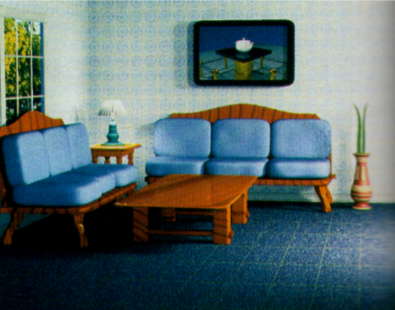
\includegraphics[width=0.38\textwidth]{Figures/Cen}
			\end{center}
	\end{figure}	
\end{frame}

%%%%%%%%%%%%%%%%%%%%%%%%%%%%%%%%%%%%%%%%%%%%%%%%%%%%%%%%%%%%%%%%%%%%%%%%%%%%%%%%%%%%%%%%%%
\section{Viewing Pipeline 3D}
\begin{frame}
\frametitle{Introdução}


	\begin{block}{Criando uma Imagem}
		\begin{itemize}
			\item O processo para criar uma imagem em computação gráfica em uma cena 3D é semelhante a tirar uma foto.
			\begin{itemize}
				\item Define-se a posição de visão da câmera.
				\item Define-se a orientação da câmera.
				\begin{itemize}
					\item Como a câmera estará apontada a partir da posição de visão.
					\item COmo a câmera vai rotacionar definindo a posição \textbf{up}.
				\end{itemize}
			\end{itemize}
		\end{itemize}
	\end{block}
	
	\begin{figure}[!h]
			\begin{center}
			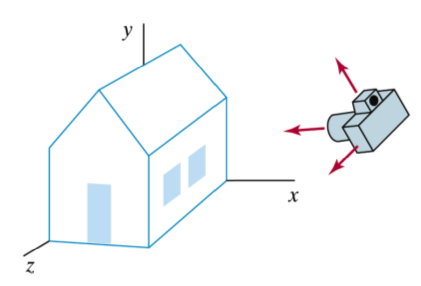
\includegraphics[width=0.5\textwidth]{Figures/CamPos}
			\end{center}
	\end{figure}	
\end{frame}

%%%%%%%%%%%%%%%%%%%%%%%%%%%%%%%%%%%%%%%%%%%%%%%%%%%%%%%%%%%%%%%%%%%%%%%%%%%%%%%%%%%%%%%%%%
\begin{frame}
\frametitle{Introdução}


	\begin{block}{Criando uma Imagem}
		\begin{itemize}
			\item<1-> Há algumas semelhanças entre o \textit{Pipeline da Viewing 2D e 3D}.
			\begin{itemize}
				\item Uma \textbf{viewport 2D} é utilizada para posicionar a visão projetada no dispositivo de saída.
				\item  Uma janela de recorte 2D é utilizada para selecionar o que será visto na cena e mapeado para viewport.
			\end{itemize}
			\item<2-> Porém há algumas diferenças
			\begin{itemize}
				\item A janela de recorte é posicionada sobre um plano de visão.
				\item A cena é recortada considerando um volume no espaço (volume de recorte) usando planos de recorte.
			\end{itemize}
		\end{itemize}
	\end{block}
\end{frame}

%%%%%%%%%%%%%%%%%%%%%%%%%%%%%%%%%%%%%%%%%%%%%%%%%%%%%%%%%%%%%%%%%%%%%%%%%%%%%%%%%%%%%%%%%%
\begin{frame}
\frametitle{Introdução}


	\begin{block}{Vieing Pipeline 3D}
		\begin{itemize}
			\item O \textbf{Plano de Visão}, \textbf{Janela de Recorte}, a \textbf{Posição da Visão} e os \textbf{Planos de Recorte} são definidos nas \textbf{coordenadas do mundo}. 
		\end{itemize}
	\end{block}
	
	\begin{figure}[!h]
			\begin{center}
			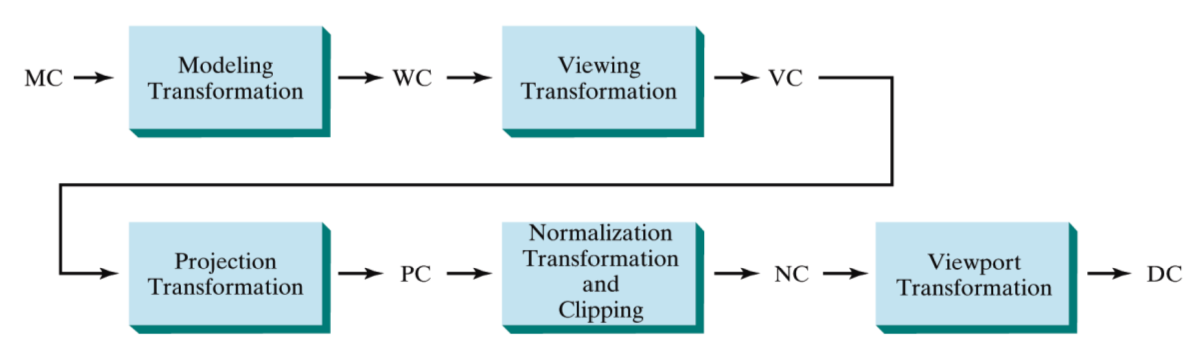
\includegraphics[width=0.9\textwidth]{Figures/3DPip}
			\end{center}
	\end{figure}
\end{frame}

%%%%%%%%%%%%%%%%%%%%%%%%%%%%%%%%%%%%%%%%%%%%%%%%%%%%%%%%%%%%%%%%%%%%%%%%%%%%%%%%%%%%%%%%%%
\section{Parâmetros de Coordenadas de Visão 3D}
\begin{frame}
\frametitle{Parâmetros de Coordenadas de Visão 3D}
	\begin{block}{Parâmetros de Coordenadas de Visão 3D}
		\begin{itemize}
			\item Para estabelecer um parâmetro de coordenadas 3D é necessário:
				\begin{itemize}
					\item A origem do sistema $ \textbf{P}_0 =(x_0,y_0,z_0)$ chamado de \textbf{Ponto de Visão}(Onde o observador ou câmera se encontra).
					\item O vetor \textbf{View up} \textbf{V}, que define a direção do $y_{view}$.
					\item Uma segunda direção para um dos eixos de orientação. Normalmente o $z_{view}$ que representa a orientação do eixo de visão.
				\end{itemize}
		\end{itemize}
	\end{block}
	
	\begin{figure}[!h]
			\begin{center}
			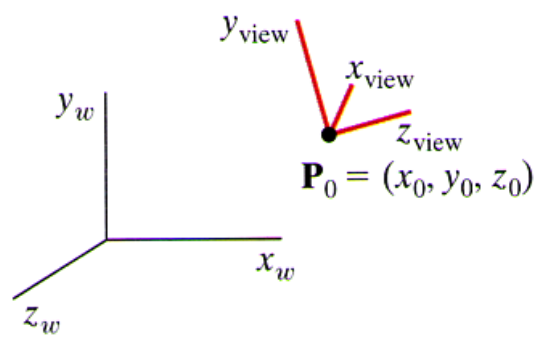
\includegraphics[width=0.48\textwidth]{Figures/3DSisCoo}
			\end{center}
	\end{figure}
\end{frame}

%%%%%%%%%%%%%%%%%%%%%%%%%%%%%%%%%%%%%%%%%%%%%%%%%%%%%%%%%%%%%%%%%%%%%%%%%%%%%%%%%%%%%%%%%%
\begin{frame}
\frametitle{Parâmetros de Coordenadas de Visão 3D}
	\begin{block}{Vetor Paralelo ao Plano}
		\begin{itemize}
			\item Geralmente o plano de visão é dado pelo eixo $z_{view}$ e o plano de projeção é formado a partir de um plano perpendicular ao eixo $z$.
			\begin{itemize}
				\item Assim a orientação do plano de projeção e a direção projetiva do eixo $z_{view}$ são dados por um vetor normal \textbf{N} ao \textbf{Plano de Projeção}. 
			\end{itemize}
		\end{itemize}
	\end{block}
	
	\begin{figure}[!h]
			\begin{center}
			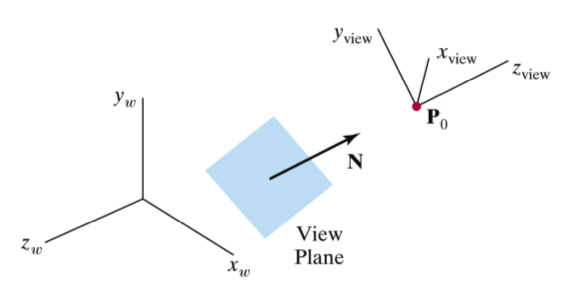
\includegraphics[width=0.7\textwidth]{Figures/PlaVie}
			\end{center}
	\end{figure}
\end{frame}

%%%%%%%%%%%%%%%%%%%%%%%%%%%%%%%%%%%%%%%%%%%%%%%%%%%%%%%%%%%%%%%%%%%%%%%%%%%%%%%%%%%%%%%%%%
\begin{frame}
\frametitle{Parâmetros de Coordenadas de Visão 3D}
	\begin{block}{Vetor Paralelo ao Plano}
		\begin{itemize}
			\item Um escalar é utilizado para definir a movimentação do plano em um ponto $z_{vp}$ ao longo do eixo $z_{view}$.
			\item O plano de visão é sempre paralelo ao plano $x_{view} \: y_{view}$.
		\end{itemize}
	\end{block}
	
	\begin{figure}[!h]
			\begin{center}
			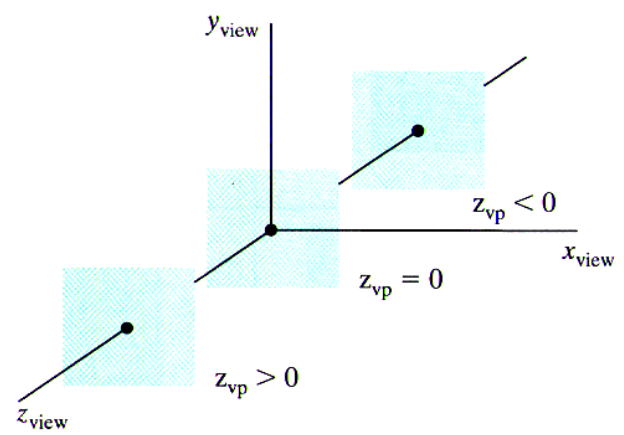
\includegraphics[width=0.6\textwidth]{Figures/MovPla}
			\end{center}
	\end{figure}
\end{frame}

%%%%%%%%%%%%%%%%%%%%%%%%%%%%%%%%%%%%%%%%%%%%%%%%%%%%%%%%%%%%%%%%%%%%%%%%%%%%%%%%%%%%%%%%%%
\begin{frame}
\frametitle{Parâmetros de Coordenadas de Visão 3D}
	\begin{block}{Vetor Paralelo ao Plano}
		\begin{itemize}
			\item O vetor normal \textbf{N} pode ser obtido de várias formas:
				\begin{itemize}
					\item A direção de \textbf{N} pode ser obtida a partir de um ponto $\textbf{P}_{ref}$ até o ponto de origem $\textbf{P}_0$ (O inverso também é válido).
					\begin{itemize}
						\item Neste caso o vetor \textbf{N} é denominado \textbf{look-at point}, com a direção oposta a visão de \textbf{N}.
					\end{itemize}
				\end{itemize}
		\end{itemize}
	\end{block}
	
	\begin{figure}[!h]
			\begin{center}
			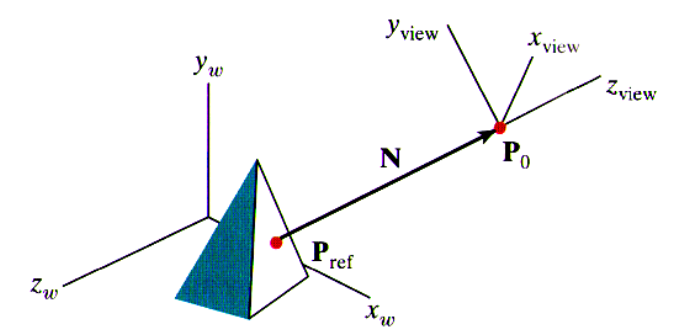
\includegraphics[width=0.6\textwidth]{Figures/VecN}
			\end{center}
	\end{figure}
\end{frame}

%%%%%%%%%%%%%%%%%%%%%%%%%%%%%%%%%%%%%%%%%%%%%%%%%%%%%%%%%%%%%%%%%%%%%%%%%%%%%%%%%%%%%%%%%%
\begin{frame}
\frametitle{Vetor View Up}
	\begin{block}{Vetor Paralelo ao Plano}
		\begin{itemize}
			\item Uma vez definida a posição e orientação do vetor \textbf{N}, é necessário encontrar o vetor \textbf{view up} V que mostra a direção do eixo $y_{view}$.
			\item Normalmente \textbf{V} é definido selecionado uma posição relativa a origem do sistema de coordenadas do mundo.
		\end{itemize}
	\end{block}
	\begin{figure}[!h]
			\begin{center}
			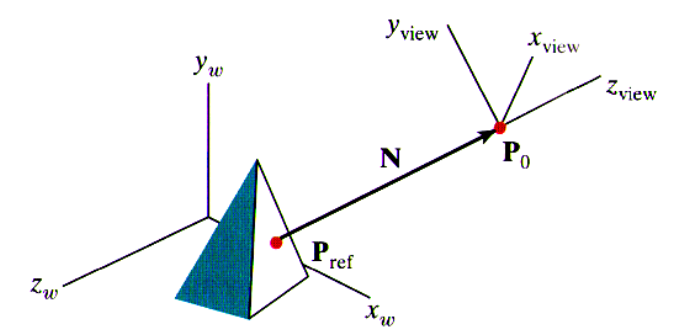
\includegraphics[width=0.6\textwidth]{Figures/VecN}
			\end{center}
	\end{figure}
\end{frame}

%%%%%%%%%%%%%%%%%%%%%%%%%%%%%%%%%%%%%%%%%%%%%%%%%%%%%%%%%%%%%%%%%%%%%%%%%%%%%%%%%%%%%%%%%%
\begin{frame}
\frametitle{Parâmetros de Coordenadas de Visão 3D}
	\begin{block}{Vetor View Up}
		\begin{itemize}
			\item O vetor \textbf{V} pode ser definido em qualquer direção exceto paralela ao vetor \textbf{N}.
			\begin{itemize}
				\item Uma forma conveniente é definir o \textbf{V} como sendo paralelo ao eixo $y$. $\textbf{V}=(0,1,0)$.
				\item Se \textbf{V} não for perpendicular a \textbf{N}, rotinas de visão podem ser aplicadas para ajustar(projetar) o vetor de modo que seja.
				\item A projeção do vetor \textbf{V} em \textbf{N} pode ser dada por:
				\begin{equation*}
					proj_{V_{imp},N} = V_{proj} = \frac{V \cdot N}{(||N||)^2} \cdot N
				\end{equation*}
				\item E o vetor $\textbf{V}_{ajust}$ pode ser encontrado utilizando soma de vetore:
					\begin{equation*}
						V_{ajust} = V_{imp} - V_{proj} 
					\end{equation*}
			\end{itemize}
			
		\end{itemize}
	\end{block}
\end{frame}

%%%%%%%%%%%%%%%%%%%%%%%%%%%%%%%%%%%%%%%%%%%%%%%%%%%%%%%%%%%%%%%%%%%%%%%%%%%%%%%%%%%%%%%%%%
\begin{frame}
\frametitle{Parâmetros de Coordenadas de Visão 3D}

	\begin{figure}[!h]
			\begin{center}
			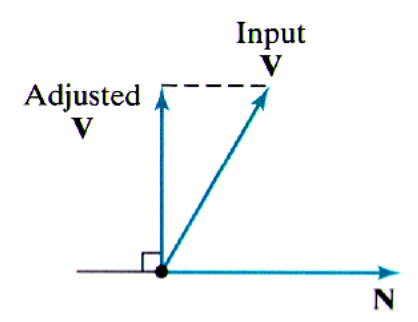
\includegraphics[width=0.6\textwidth]{Figures/VecPro}
			\caption{Ajuste do vetor \textbf{view up} para torna-lo perpendicular a \textbf{N}}
			\end{center}
	\end{figure}

\end{frame}

%%%%%%%%%%%%%%%%%%%%%%%%%%%%%%%%%%%%%%%%%%%%%%%%%%%%%%%%%%%%%%%%%%%%%%%%%%%%%%%%%%%%%%%%%%
\begin{frame}
\frametitle{Sistema de Coordenadas de Visão $u \times n$}
	\begin{block}{Sistema de Coordenadas de Visão $u \times n$}
		\begin{itemize}
			\item Com o vetor normal \textbf{N} definido, assim como o vetor view up \textbf{V}, basta apenas encontrar a direção positiva do eixo $x_{view}$.
			\begin{itemize}
				\item A direção de $x_{view}$ é representada por um vetor \textbf{U} obtido a partir do produto vetorial de \textbf{N} e \textbf{V}
				\item O produto vetorial entre \textbf{N} e \textbf{U} também pode ser utilizado para ajustar \textbf{V} no eixo $y_{view}$.
			\end{itemize}
		\end{itemize}
	\end{block}
\end{frame}

%%%%%%%%%%%%%%%%%%%%%%%%%%%%%%%%%%%%%%%%%%%%%%%%%%%%%%%%%%%%%%%%%%%%%%%%%%%%%%%%%%%%%%%%%%
\begin{frame}
\frametitle{Sistema de Coordenadas de Visão $u \times n$}
	\begin{block}{Sistema de Coordenadas de Visão $u \times n$}
		\begin{itemize}
			\item Para se obter o sistema de coordenadas \textbf{uvn} é necessário:
				\begin{eqnarray*}
					n = \frac{N}{|N|} = (n_x,n_y,n_z) \\
					u = \frac{V \times n}{|V \times n|} = (u_x,u_y,u_z) \\
					v = n \times u = (v_x,v_y,v_z)
				\end{eqnarray*}
		\end{itemize}
	\end{block}
	
	\begin{figure}[!h]
			\begin{center}
			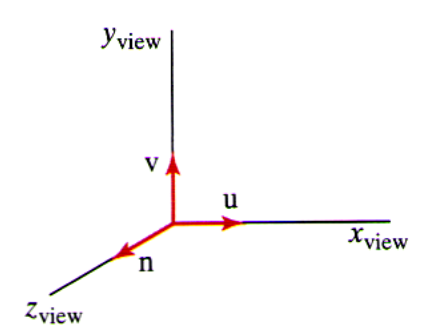
\includegraphics[width=0.38\textwidth]{Figures/uvn}
			\end{center}
	\end{figure}
\end{frame}


%%%%%%%%%%%%%%%%%%%%%%%%%%%%%%%%%%%%%%%%%%%%%%%%%%%%%%%%%%%%%%%%%%%%%%%%%%%%%%%%%%%%%%%%%%
\begin{frame}
\frametitle{Gerando Efeitos de Visão 3D}
	\begin{block}{Gerando Efeitos de Visão 3D}
		\begin{itemize}
			\item Variando alguns parâmetros de visão é possível obter vários efeitos 3D.
				\begin{itemize}
					\item De uma posição fixa é possível variar \textbf{N} de forma que seja possível observar objetos ao redor da posição.
					\item Variar \textbf{N} para obter uma cena composta de múltiplas visões de uma posição fixa da câmera.
					\begin{itemize}
						\item Lembrando que para cada posição de \textbf{N} é necessário ajustar os vetores dos eixos restantes mantendo a regra da mão direita.
					\end{itemize}
				\end{itemize}
		\end{itemize}
	\end{block}
	
	\begin{figure}[!h]
			\begin{center}
			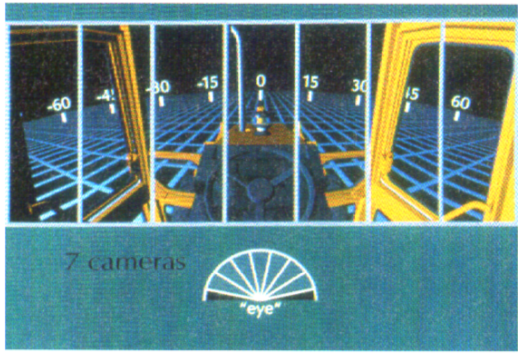
\includegraphics[width=0.38\textwidth]{Figures/MulN}
			\end{center}
	\end{figure}
\end{frame}

%%%%%%%%%%%%%%%%%%%%%%%%%%%%%%%%%%%%%%%%%%%%%%%%%%%%%%%%%%%%%%%%%%%%%%%%%%%%%%%%%%%%%%%%%%
\begin{frame}
\frametitle{Gerando Efeitos de Visão 3D}
	\begin{block}{Gerando Efeitos de Visão 3D}
		\begin{itemize}
			\item Efeitos de movimento da câmera (pam) podem ser obtidos fixando \textbf{N} e modificando a posição da câmera.
			\item Para mostrar diferentes visões de um objeto podemos mover o ponto de visão ao redor do objeto.
		\end{itemize}
	\end{block}
	
	\begin{figure}[!h]
			\begin{center}
			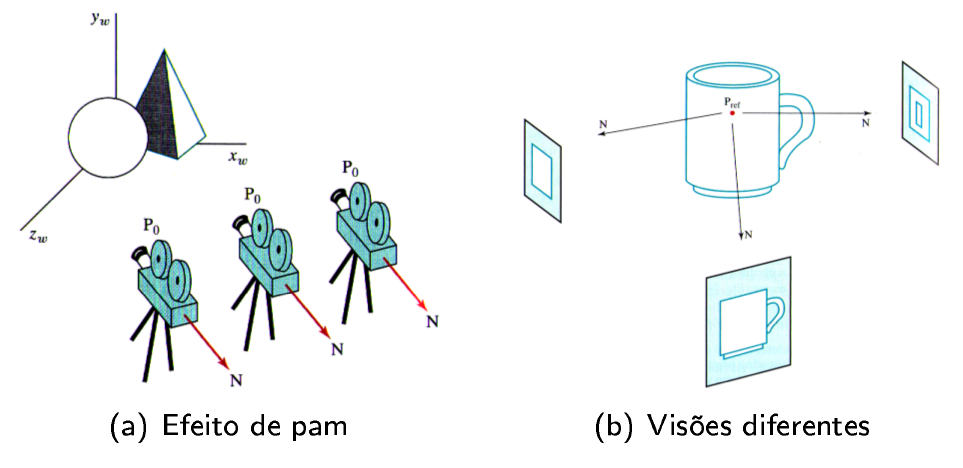
\includegraphics[width=0.8\textwidth]{Figures/camEfe}
			\end{center}
	\end{figure}
\end{frame}


%%%%%%%%%%%%%%%%%%%%%%%%%%%%%%%%%%%%%%%%%%%%%%%%%%%%%%%%%%%%%%%%%%%%%%%%%%%%%%%%%%%%%%%%%%
\section{Transformação das Coordenadas do Mundo para as de Visão}
\begin{frame}
\frametitle{Transformação das Coordenadas do Mundo para as de Visão}
	\begin{block}{Transformação das Coordenadas do Mundo para as de Visão}
		\begin{itemize}
			\item No \textbf{Viewing Pipeline 3D} o próximo passo a ser executado após a cena ser montada é transferir as coordenadas dos objetos para para o sistema de coordenadas de visão.
			\begin{itemize}
				\item Há uma sobreposição do sistema de coordenadas de visão sobre o sistema de coordenadas do mundo.
			\end{itemize}
			\item Esta conversão é dada por:
				\begin{enumerate}
					\item Translada-se a origem do sistema de visão para a origem do sistema de coordenadas do mundo.
					\item Rotaciona os eixos $x_{view},y_{view}$ e $z_{view}$ para deixa-los alinhados com os eixos $x_{wc},y_{wc}$ e $z_{wc}$.
				\end{enumerate}
		\end{itemize}
	\end{block}
\end{frame}



%%%%%%%%%%%%%%%%%%%%%%%%%%%%%%%%%%%%%%%%%%%%%%%%%%%%%%%%%%%%%%%%%%%%%%%%%%%%%%%%%%%%%%%%%%
\begin{frame}
\frametitle{Transformação das Coordenadas do Mundo para as de Visão}
	\begin{block}{Transformação das Coordenadas do Mundo para as de Visão}
		\begin{itemize}
			\item Se a origem do sistema de visão for em $P_0(x_0,y_0,z_0)$ a matriz de translação \textbf{T} será:
			\begin{equation*}
				\textbf{T} = \begin{bmatrix}
					1	&	0	&	0	&	-x_0	\\
					0	&	1	&	0	&	-y_0\\
					0	&	0	&	1	&	-z_0\\
					0	&	0	&	0	&	1
				\end{bmatrix}
			\end{equation*}
		\end{itemize}
	\end{block}
\end{frame}


%%%%%%%%%%%%%%%%%%%%%%%%%%%%%%%%%%%%%%%%%%%%%%%%%%%%%%%%%%%%%%%%%%%%%%%%%%%%%%%%%%%%%%%%%%
\begin{frame}
\frametitle{Transformação das Coordenadas do Mundo para as de Visão}
	\begin{block}{Transformação das Coordenadas do Mundo para as de Visão}
		\begin{itemize}
			\item A Matriz de Rotação poder ser obtida por meio dos vetores $\textbf{u}=(u_x,u_y,u_z),\textbf{v}=(v_x,v_y,v_z)$ e $\textbf{n}=(n_x,n_y,n_z)$:
			\begin{equation*}
				\textbf{R} = \begin{bmatrix}
					u_x	&	u_y	&	u_z	&	0	\\
					v_x	&	v_y	&	v_z	&	0	\\
					n_x	&	n_y	&	n_z	&	0	\\
					0	&	0	&	0	&	1
				\end{bmatrix}
			\end{equation*}
		\end{itemize}
	\end{block}
\end{frame}


%%%%%%%%%%%%%%%%%%%%%%%%%%%%%%%%%%%%%%%%%%%%%%%%%%%%%%%%%%%%%%%%%%%%%%%%%%%%%%%%%%%%%%%%%%
\begin{frame}
\frametitle{Transformação das Coordenadas do Mundo para as de Visão}
	\begin{block}{Transformação das Coordenadas do Mundo para as de Visão}
		\begin{itemize}
			\item Portanto a matriz de transformação é:
			\begin{equation*}
				\textbf{M}_{WC,VC} = R \cdot T  = \begin{bmatrix}
					u_x	&	u_y	&	u_z	&	-u \cdot P_0	\\
					v_x	&	v_y	&	v_z	&	-v \cdot P_0	\\
					n_x	&	n_y	&	n_z	&	-z \cdot P_0	\\
					0	&	0	&	0	&	1
				\end{bmatrix}
			\end{equation*}
		\end{itemize}
	\end{block}
\end{frame}


%%%%%%%%%%%%%%%%%%%%%%%%%%%%%%%%%%%%%%%%%%%%%%%%%%%%%%%%%%%%%%%%%%%%%%%%%%%%%%%%%%%%%%%%%%
\section{Transformação de Projeções}

\begin{frame}
\frametitle{Transformações de Projeção}
	\begin{block}{Transformações de Projeção}
		\begin{itemize}
			\item Após a transformação para as coordenadas de visão, o próximo passo do Viewing Pipeline 3D é a projeção no plano de projeção.
		\end{itemize}
	\end{block}

	\begin{block}{Pacotes Gráficos}
		\begin{itemize}
			\item Em geral os pacotes gráficos suportam:
				\begin{itemize}
					\item \textbf{Projeção Paralela}: as coordenadas são transferidas para o plano de projeção ao longo de linhas paralelas.
					\item \textbf{Projeção Perspectiva}: as coordenadas são transferidas para um ponto convergindo para um ponto.
				\end{itemize}
		\end{itemize}
	\end{block}
\end{frame}


%%%%%%%%%%%%%%%%%%%%%%%%%%%%%%%%%%%%%%%%%%%%%%%%%%%%%%%%%%%%%%%%%%%%%%%%%%%%%%%%%%%%%%%%%%
\begin{frame}
\frametitle{Transformações de Projeção}
	\begin{figure}[!h]
			\begin{center}
			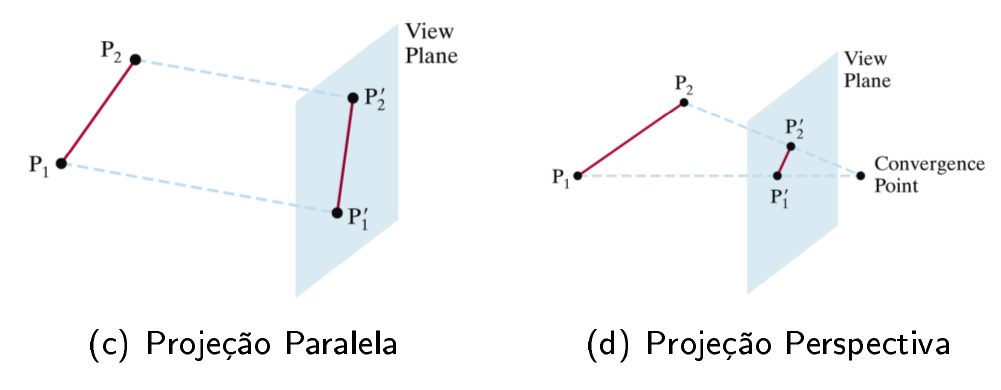
\includegraphics[width=0.9\textwidth]{Figures/TipProj}
			\end{center}
	\end{figure}
\end{frame}

%%%%%%%%%%%%%%%%%%%%%%%%%%%%%%%%%%%%%%%%%%%%%%%%%%%%%%%%%%%%%%%%%%%%%%%%%%%%%%%%%%%%%%%%%%

\subsection{Projeções Ortogonais}
\begin{frame}
\frametitle{Projeções Ortogonais ou Ortográficas}
	\begin{block}{Projeções Ortogonais}
		\begin{itemize}
			\item Transformam as descrições dos objetos utilizando um plano de projeção ao longo das linhas paralelas ao ao vetor \textbf{N}.
			\item É utilizada para visão frontal, lateral e superior dos objetos.
			\item Preserva o tamanho e ângulos dos objetos. Devido a isso este tipo de projeção é principalmente utilizada em programas arquitetônicos.
		\end{itemize}
	\end{block}
	
	\begin{figure}[!h]
			\begin{center}
			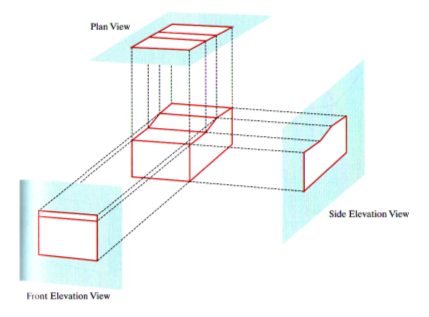
\includegraphics[width=0.4\textwidth]{Figures/ProjOrt}
			\end{center}
	\end{figure}
\end{frame}

%%%%%%%%%%%%%%%%%%%%%%%%%%%%%%%%%%%%%%%%%%%%%%%%%%%%%%%%%%%%%%%%%%%%%%%%%%%%%%%%%%%%%%%%%%
\begin{frame}
\frametitle{Projeções Ortogonais ou Ortográficas}
	\begin{block}{Projeções Axonométricas}
		\begin{itemize}
			\item É a projeção ortogonal que mostras mais de uma face do objeto.
		\end{itemize}
	\end{block}
	
	\begin{block}{Projeções Axonométricas Isométrica}
		\begin{itemize}
			\item A projeção \textbf{Isométrica} é a projeção Axonométrica mais comum.
				\begin{itemize}
					\item Ela consiste em alinhar o plano de projeção de forma a intersectar cada eixo coordenado no qual o objeto é definido a mesma distância da origem.
				\end{itemize}
		\end{itemize}
	\end{block}	
	
	\begin{figure}[!h]
			\begin{center}
			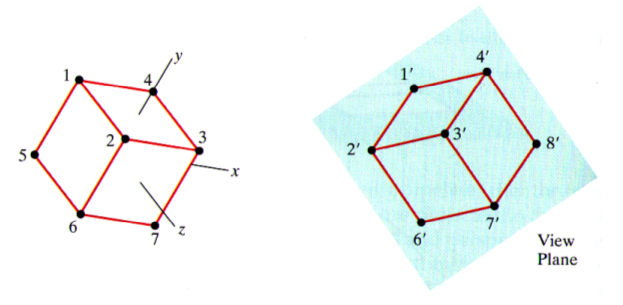
\includegraphics[width=0.4\textwidth]{Figures/ProIso}
			\caption{Esta projeção é obtida alinhando o vetor \textbf{N} com a diagonal do cubo.}
			\end{center}
	\end{figure}
\end{frame}


%%%%%%%%%%%%%%%%%%%%%%%%%%%%%%%%%%%%%%%%%%%%%%%%%%%%%%%%%%%%%%%%%%%%%%%%%%%%%%%%%%%%%%%%%%
\begin{frame}
\frametitle{Projeções Ortogonais ou Ortográficas}
	\begin{block}{Coordenadas de Projeções Ortogonais}
		\begin{itemize}
			\item Com a direção do da projeção sendo paralela ao eixo $z_{view}$, as equações para as transformações de projeção ortogonal em uma posição $(x,y,z)$ são:
			\begin{eqnarray*}
				x_p = x \\
				y_p = y
			\end{eqnarray*}
			\item O valor de $z$ é armazenado para futuras procedimentos para determinar a visibilidade.
		\end{itemize}
	\end{block}
	\begin{figure}[!h]
			\begin{center}
			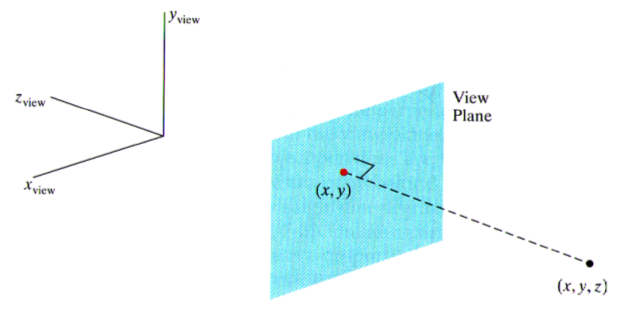
\includegraphics[width=0.4\textwidth]{Figures/PlaProOrt}
			\end{center}
	\end{figure}
\end{frame}

%%%%%%%%%%%%%%%%%%%%%%%%%%%%%%%%%%%%%%%%%%%%%%%%%%%%%%%%%%%%%%%%%%%%%%%%%%%%%%%%%%%%%%%%%%
\begin{frame}
\frametitle{Projeções Ortogonais ou Ortográficas}
	\begin{block}{Janela de Recorte e Volume de Projeção Ortogonal}
		\begin{itemize}
			\item Para determinar o quando da cena aparecerá, uma janela de recorte é então utilizada.
			\begin{itemize}
				\item É necessário determinar os limites da janela de projeção sobre o plano formado pelos eixos $x_{view} \times y_{view}$, ou seja, com as arestas paralelas aos mesmos.
			\end{itemize}
		\end{itemize}
	\end{block}
	\begin{figure}[!h]
			\begin{center}
			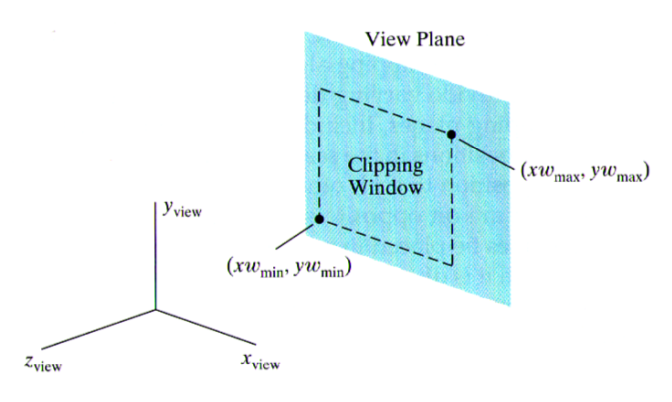
\includegraphics[width=0.7\textwidth]{Figures/PlaProXY}
			\end{center}
	\end{figure}
\end{frame}


%%%%%%%%%%%%%%%%%%%%%%%%%%%%%%%%%%%%%%%%%%%%%%%%%%%%%%%%%%%%%%%%%%%%%%%%%%%%%%%%%%%%%%%%%%
\begin{frame}
\frametitle{Projeções Ortogonais ou Ortográficas}
	\begin{block}{Janela de Recorte e Volume de Projeção Ortogonal}
		\begin{itemize}
			\item As arestas da \textbf{Janela de Recorte} especificam os valores de $x$ e $y$ que serão mostrados na cena, formando assim, o \textbf{Volume de Visão de Projeção Ortogonal}.
		\end{itemize}
	\end{block}
	\begin{figure}[!h]
			\begin{center}
			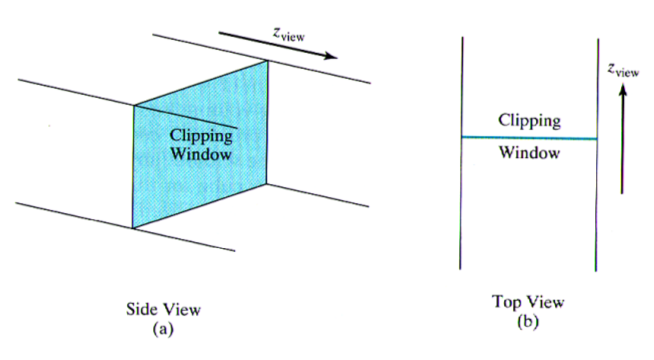
\includegraphics[width=0.7\textwidth]{Figures/VolOrt}
			\end{center}
	\end{figure}
\end{frame}


%%%%%%%%%%%%%%%%%%%%%%%%%%%%%%%%%%%%%%%%%%%%%%%%%%%%%%%%%%%%%%%%%%%%%%%%%%%%%%%%%%%%%%%%%%
\begin{frame}
\frametitle{Projeções Ortogonais ou Ortográficas}
	\begin{block}{Janela de Recorte e Volume de Projeção Ortogonal}
		\begin{itemize}
			\item Para limitar a extensão do volume de projeção dois planos de fronteira, denominados \textbf{Planos de Recorte Near/Far} são utilizados paralelamente aos planos de visão.
			\begin{itemize}
				\item Permite eliminar objetos que estão na frente ou atrás de uma parte da cena.
				\item Com a direção de visão ao longo do eixo negativo de $z_{view}$, temos $z_{far} < z_{near}$.
			\end{itemize}
		\end{itemize}
	\end{block}
	\begin{figure}[!h]
			\begin{center}
			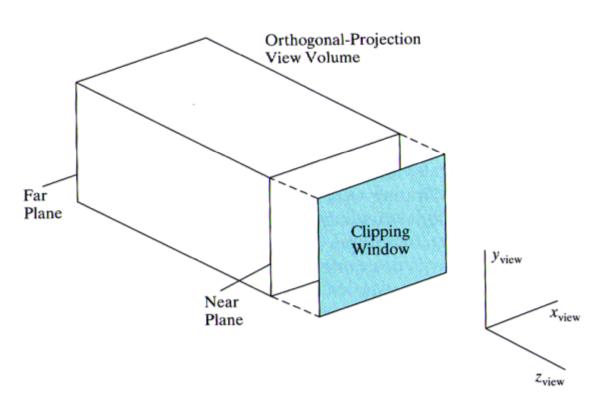
\includegraphics[width=0.5\textwidth]{Figures/FarNea}
			\end{center}
	\end{figure}
\end{frame}


%%%%%%%%%%%%%%%%%%%%%%%%%%%%%%%%%%%%%%%%%%%%%%%%%%%%%%%%%%%%%%%%%%%%%%%%%%%%%%%%%%%%%%%%%%
\begin{frame}
\frametitle{Projeções Ortogonais ou Ortográficas}
	\begin{block}{Transformações de Normalização para Projeção Ortogonal}
		\begin{itemize}
			\item Qualquer posição $(x,y,z)$ em uma projeção ortogonal pode ser mapeada para $(x,y)$, as coordenadas dentro do volume de visão são as coordenadas de projeção, assim elas podem ser mapeadas para o \textbf{volume de visão normalizado} sem precisar ser reprojetadas.
		\end{itemize}
	\end{block}
	\begin{figure}[!h]
			\begin{center}
			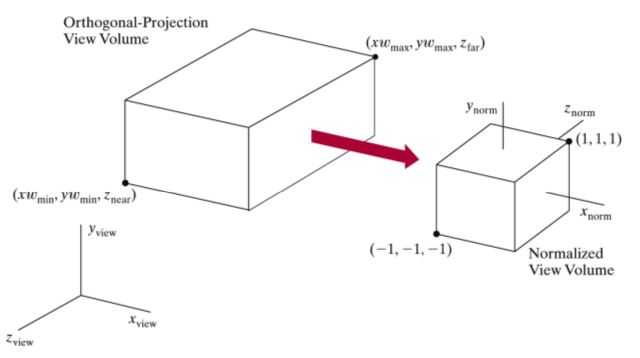
\includegraphics[width=0.5\textwidth]{Figures/ProNor}
			\caption{Transformações de normalização de um sistema de referência baseado na regra da mão esquerda.}
			\end{center}
	\end{figure}
\end{frame}

%%%%%%%%%%%%%%%%%%%%%%%%%%%%%%%%%%%%%%%%%%%%%%%%%%%%%%%%%%%%%%%%%%%%%%%%%%%%%%%%%%%%%%%%%%
\begin{frame}
\frametitle{Projeções Ortogonais ou Ortográficas}
	\begin{block}{Transformações de Normalização para Projeção Ortogonal}
		\begin{itemize}
			\item A transformação de normalização é semelhante a obtida em 2D, com a adição da coordenada $z$ normalizada no intervalo $z_{near}$ a $z_{far}$ para -1 e 1:
			\begin{eqnarray*}
				\textbf{M}_{ortho,norm} = R \cdot T  \\
					= \begin{bmatrix}
					\frac{2}{xw_{max} - xw_{min}}	&	0								&	0								&	- \frac{xw_{max}+xw_{min}}{xw_{max}-xw_{min}}	\\
					0								&	\frac{2}{yw_{max} - yw_{min}}	&	0								&	- \frac{yw_{max}+yw_{min}}{yw_{max}-yw_{min}}	\\
					0								&	0								&	\frac{-2}{z_{near} - z_{far}}	&	- \frac{z_{far}+z_{near}}{z_{far}-z_{near}}\\
					0								&	0	&	0	&	1
				\end{bmatrix}
			\end{eqnarray*}
		\end{itemize}
	\end{block}
\end{frame}

%%%%%%%%%%%%%%%%%%%%%%%%%%%%%%%%%%%%%%%%%%%%%%%%%%%%%%%%%%%%%%%%%%%%%%%%%%%%%%%%%%%%%%%%%%
\begin{frame}
\frametitle{Projeções Ortogonais ou Ortográficas}
	\begin{block}{Transformações de Normalização para Projeção Ortogonal}
		\begin{itemize}
			\item A multiplicação desta matriz com a matriz que transforma as coordenadas do mundo em coordenadas de visão produz a transformação correta para se obter as coordenadas corretas para se obter as coordenadas normalizadas da projeção ortogonal.
			\begin{equation*}
				\textbf{M}_{ortho,norm} \cdot \textbf{M}_{WC,VC}
			\end{equation*}
			
			\item Com a normalização operações como a de recorte e identificação se superfícies visíveis podem ser feitas de modo mais eficiente.
		\end{itemize}
	\end{block}
\end{frame}

%%%%%%%%%%%%%%%%%%%%%%%%%%%%%%%%%%%%%%%%%%%%%%%%%%%%%%%%%%%%%%%%%%%%%%%%%%%%%%%%%%%%%%%%%%
\subsection{Projeções Perspectivas}
\begin{frame}
\frametitle{Projeções Perspectivas}
	\begin{block}{Projeções Perspectivas}
		\begin{itemize}
			\item Para um maior realismo nas cenas, quando comparado a perspectiva, temos que levar em consideração que os raios de luz refletidos na cena possuem caminhos convergentes.
			\item Uma aproximação desta característica pode ser feita projetando os objetos ao plano de visão ao longo de caminhos convergentes a uma posição chamada \textbf{ponto de referência de projeção (centro da projeção)}.
		\end{itemize}
	\end{block}
	
	\begin{figure}[!h]
			\begin{center}
			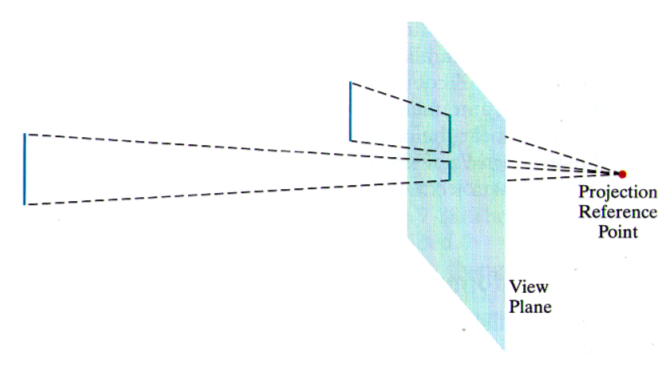
\includegraphics[width=0.5\textwidth]{Figures/PonPro}
			\end{center}
	\end{figure}
\end{frame}

%%%%%%%%%%%%%%%%%%%%%%%%%%%%%%%%%%%%%%%%%%%%%%%%%%%%%%%%%%%%%%%%%%%%%%%%%%%%%%%%%%%%%%%%%%
\begin{frame}
\frametitle{Transformações de Coordenadas de Projeção Perspectiva}
	\begin{block}{Transformações de Coordenadas de Projeção Perspectiva}
		\begin{itemize}
			\item Algumas bibliotecas gráficas permitem escolher o ponto de projeção $(x_{prp},y_{prp},z_{prp})$
		\end{itemize}
	\end{block}
	
	\begin{figure}[!h]
			\begin{center}
			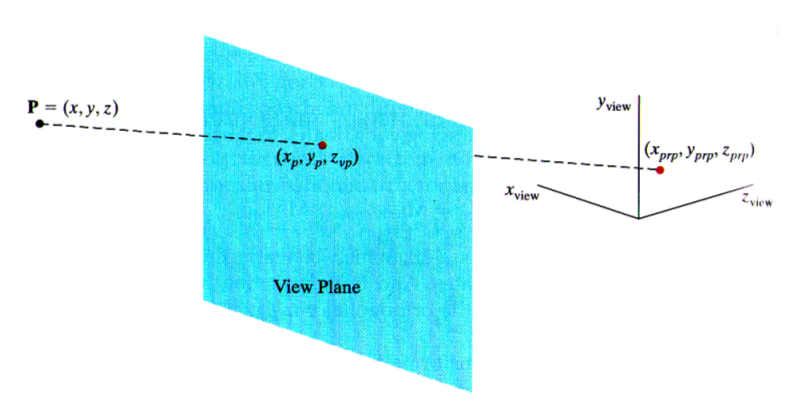
\includegraphics[width=0.8\textwidth]{Figures/PonPro2}
			\end{center}
	\end{figure}
\end{frame}


%%%%%%%%%%%%%%%%%%%%%%%%%%%%%%%%%%%%%%%%%%%%%%%%%%%%%%%%%%%%%%%%%%%%%%%%%%%%%%%%%%%%%%%%%%
\begin{frame}
\frametitle{Transformações de Coordenadas de Projeção Perspectiva}
	\begin{block}{Transformações de Coordenadas de Projeção Perspectiva}
		\begin{itemize}
			\item Considerando que a projeção do ponto $(x,y,z)$ intersecta o plano de projeção na posição $(x_p,y_p,z_p)$, podemos descrever qualquer ponto ao longo desta linha de projeção como sendo:
			\begin{eqnarray*}
				x' = x +t(x_{prp}-x) \\
				y' = y +t(y_{prp}-y) \\
				z' = z +t(z_{prp}-z) \\
				0 \leq t \leq 1
			\end{eqnarray*}
		
		\item No plano de visão $z' = z_{vp}$, então podemos encontrar $t$:
		\begin{equation*}
			t = \frac{z_{vp} - z}{z_{prp}-z}
		\end{equation*}
		\end{itemize}	
	\end{block}
\end{frame}

%%%%%%%%%%%%%%%%%%%%%%%%%%%%%%%%%%%%%%%%%%%%%%%%%%%%%%%%%%%%%%%%%%%%%%%%%%%%%%%%%%%%%%%%%%
\begin{frame}
\frametitle{Transformações de Coordenadas de Projeção Perspectiva}
	\begin{block}{Transformações de Coordenadas de Projeção Perspectiva}
		\begin{itemize}
			\item Substituindo o valor de $t$ nas equações de $x'$ e $y'$ obtemos as equações de projeção perspectiva.
		\end{itemize}	
	\end{block}
\end{frame}

%%%%%%%%%%%%%%%%%%%%%%%%%%%%%%%%%%%%%%%%%%%%%%%%%%%%%%%%%%%%%%%%%%%%%%%%%%%%%%%%%%%%%%%%%%
\begin{frame}
\frametitle{Transformações de Coordenadas de Projeção Perspectiva}
	\begin{block}{Posição do Ponto de Projeção}
		\begin{itemize}
			\item Geralmente o ponto de projeção está entre o plano de projeção e a cena, mas existem outras posições possíveis (menos sobre o plano de projeção).
		\end{itemize}	
	\end{block}
	
	\begin{figure}[!h]
			\begin{center}
			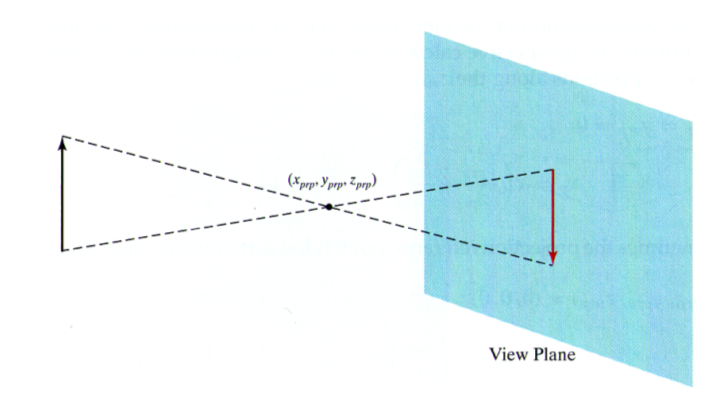
\includegraphics[width=0.6\textwidth]{Figures/PonProFre}
			\caption{Os objetos da cena será invertidos caso o ponto de referência esteja a frente do plano.}
			\end{center}
	\end{figure}
	
\end{frame}

%%%%%%%%%%%%%%%%%%%%%%%%%%%%%%%%%%%%%%%%%%%%%%%%%%%%%%%%%%%%%%%%%%%%%%%%%%%%%%%%%%%%%%%%%%
\begin{frame}
\frametitle{Transformações de Coordenadas de Projeção Perspectiva}
	\begin{block}{Posição do Ponto de Projeção}
		\begin{itemize}
			\item Os efeitos de perspectiva dependem da posição em que o centro de projeção está em relação ao plano de visão.
		\end{itemize}	
	\end{block}
	
	\begin{figure}[!h]
			\begin{center}
			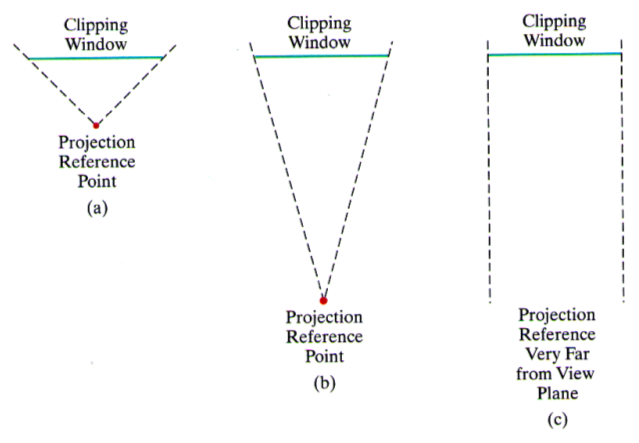
\includegraphics[width=0.6\textwidth]{Figures/PonProPos2}
			\caption{Quanto mais perto o centro de projeção está do plano, maiores serão os objetos próximos ao plano.}
			\end{center}
	\end{figure}
\end{frame}

%%%%%%%%%%%%%%%%%%%%%%%%%%%%%%%%%%%%%%%%%%%%%%%%%%%%%%%%%%%%%%%%%%%%%%%%%%%%%%%%%%%%%%%%%%
\begin{frame}
\frametitle{Transformações de Coordenadas de Projeção Perspectiva}
	\begin{block}{Pontos de Fuga na Projeção Perspectiva}
		\begin{itemize}
			\item Linhas paralelas entre si e ao plano de projeção são projetadas como linhas paralelas.
			\item Linhas paralelas que não são paralelas ao plano de projeção são projetadas em linhas convergentes.
			\item O ponto em que as Linhas convergem é denominado \textbf{Ponto de Fuga}.
		\end{itemize}	
	\end{block}
	
	\begin{figure}[!h]
			\begin{center}
			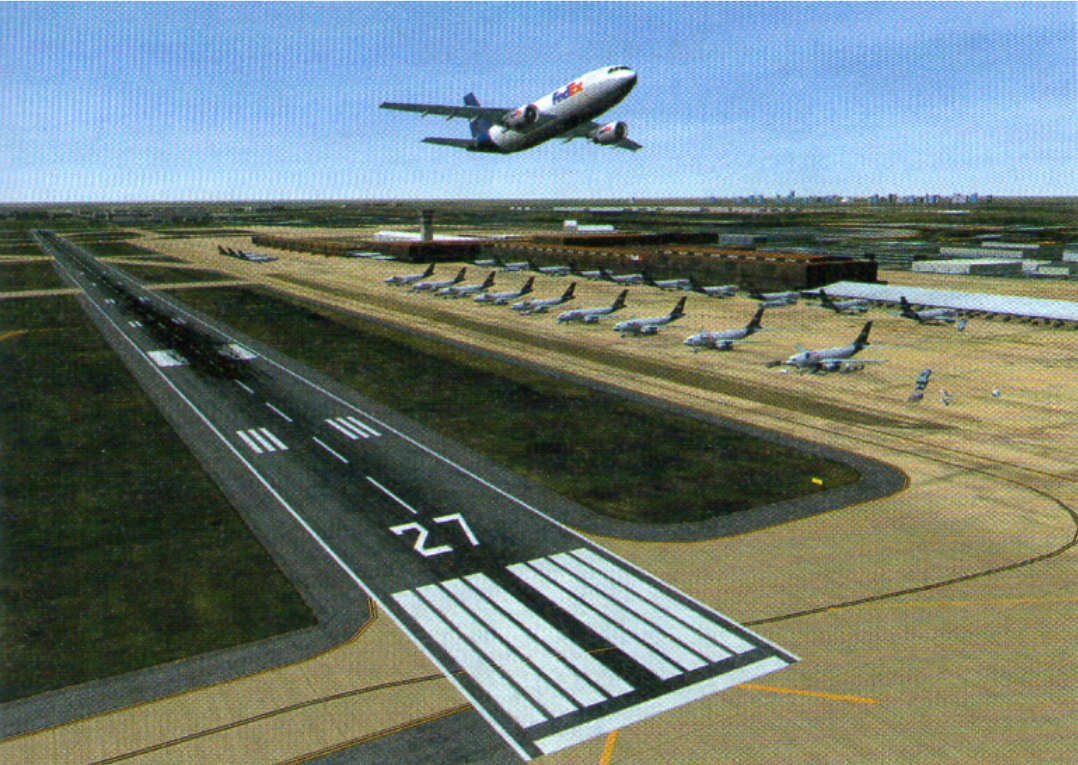
\includegraphics[width=0.55\textwidth]{Figures/Pla}
			\end{center}
	\end{figure}
\end{frame}

%%%%%%%%%%%%%%%%%%%%%%%%%%%%%%%%%%%%%%%%%%%%%%%%%%%%%%%%%%%%%%%%%%%%%%%%%%%%%%%%%%%%%%%%%%
\begin{frame}
\frametitle{Transformações de Coordenadas de Projeção Perspectiva}
	\begin{block}{Pontos de Fuga na Projeção Perspectiva}
		\begin{itemize}
			\item Os conjuntos de linhas que são paralelas ao algum dos eixos principais dos objetos levam a composição de \textbf{pontos de fuga principais}.
			\begin{itemize}
				\item É possível controlar os número de pontos de fuga, que podem ser 1,2 ou 3. Para tal controle basta mudar a orientação do plano de projeção.
				\item O número de pontos de fufa principais é igual a quantidade de eixo principais do objeto que intersectam o plano de projeção.
			\end{itemize}
		\end{itemize}	
	\end{block}
\end{frame}

%%%%%%%%%%%%%%%%%%%%%%%%%%%%%%%%%%%%%%%%%%%%%%%%%%%%%%%%%%%%%%%%%%%%%%%%%%%%%%%%%%%%%%%%%%
\begin{frame}
\frametitle{Transformações de Coordenadas de Projeção Perspectiva}
	\begin{figure}[!h]
			\begin{center}
			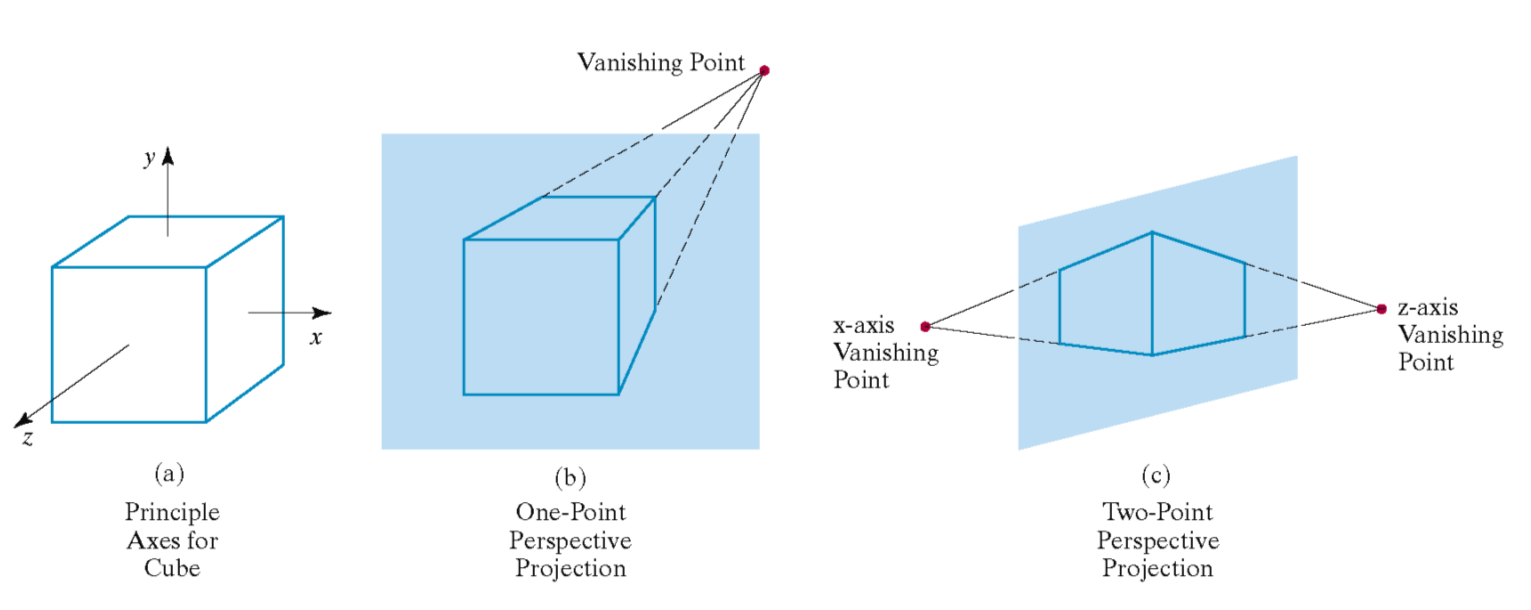
\includegraphics[width=0.8\textwidth]{Figures/PonFug}
			\caption{Em (b) o plano xy é paralelo ao plano(apenas z é intersectado), e em (c) os eixos x e y são intersectados.}
			\end{center}
	\end{figure}
\end{frame}

%%%%%%%%%%%%%%%%%%%%%%%%%%%%%%%%%%%%%%%%%%%%%%%%%%%%%%%%%%%%%%%%%%%%%%%%%%%%%%%%%%%%%%%%%%
\begin{frame}
\frametitle{Transformações de Coordenadas de Projeção Perspectiva}
	\begin{block}{Volume de Projeção Perspectiva}
		\begin{itemize}
			\item Na projeção em perspectiva, o volume de visão é definido por uma pirâmide infinita com o ápice no ponto que corresponde ao centro de projeção. Esta pirâmide é normalmente chamada de \textbf{Pirâmide de Visão}.
			\begin{itemize}
				\item Objetos estão fora dos limites da pirâmide são excluídos das rotinas de recortes.
			\end{itemize}
		\end{itemize}	
	\end{block}
	
		\begin{figure}[!h]
			\begin{center}
			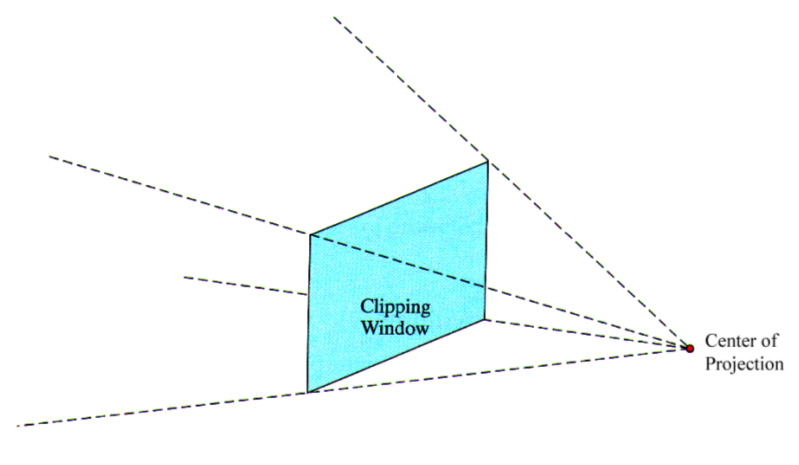
\includegraphics[width=0.5\textwidth]{Figures/VolPir}
			\end{center}
	\end{figure}
\end{frame}

%%%%%%%%%%%%%%%%%%%%%%%%%%%%%%%%%%%%%%%%%%%%%%%%%%%%%%%%%%%%%%%%%%%%%%%%%%%%%%%%%%%%%%%%%%
\begin{frame}
\frametitle{Transformações de Coordenadas de Projeção Perspectiva}
	\begin{block}{Volume de Projeção Perspectiva}
		\begin{itemize}
			\item Adicionando os planos de recorte near/far perpendiculares ao eixo $z_{view}$ a pirâmide de visão é truncada resultando em um tronco de pirâmide denominado \textbf{Frustrum}.
		\end{itemize}	
	\end{block}
	
		\begin{figure}[!h]
			\begin{center}
			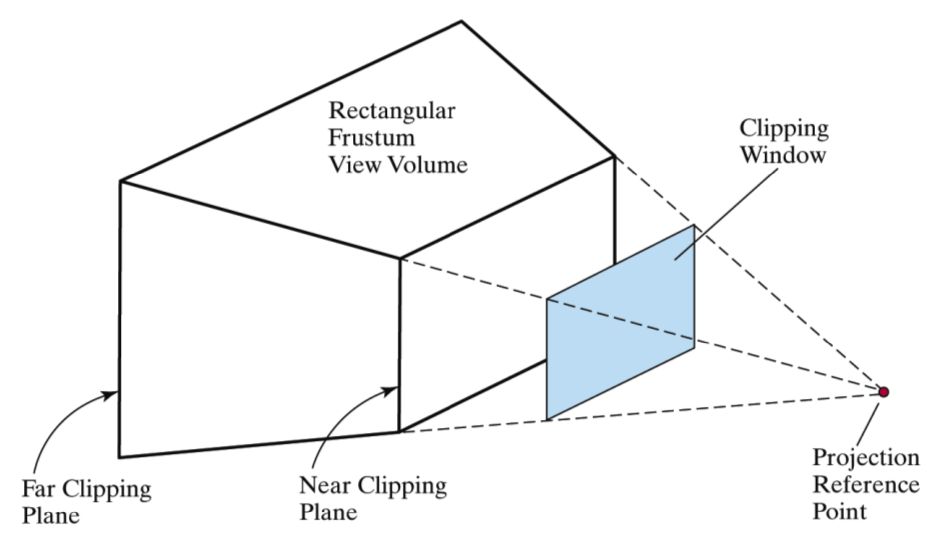
\includegraphics[width=0.8\textwidth]{Figures/Fru}
			\end{center}
	\end{figure}
\end{frame}


%%%%%%%%%%%%%%%%%%%%%%%%%%%%%%%%%%%%%%%%%%%%%%%%%%%%%%%%%%%%%%%%%%%%%%%%%%%%%%%%%%%%%%%%%%
\begin{frame}
\frametitle{Transformações de Coordenadas de Projeção Perspectiva}
	\begin{block}{Frustrum Simétrico}
		\begin{itemize}
			\item Se a linha que parte do centro de projeção  e cruza o centro da janela de recorte intersectando a linha central do Frustrum de projeção e perspectiva.
			\begin{itemize}
				\item Se essa linha for perpendicular ao plano de visão então o Frustrum é simétrico.
			\end{itemize}
		\end{itemize}	
	\end{block}
	
		\begin{figure}[!h]
			\begin{center}
			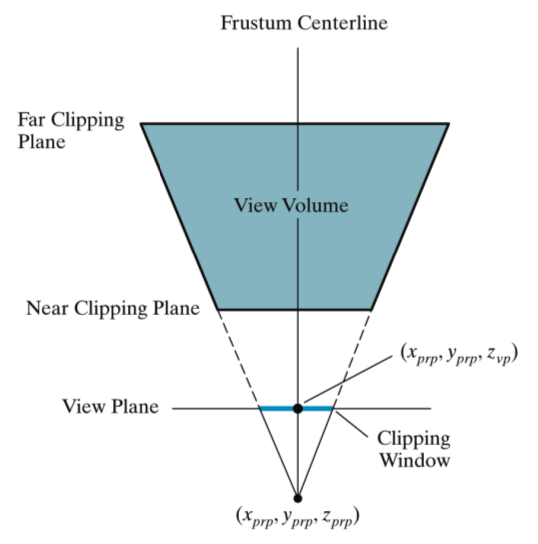
\includegraphics[width=0.4\textwidth]{Figures/FruCim}
			\end{center}
	\end{figure}
\end{frame}

%%%%%%%%%%%%%%%%%%%%%%%%%%%%%%%%%%%%%%%%%%%%%%%%%%%%%%%%%%%%%%%%%%%%%%%%%%%%%%%%%%%%%%%%%%
\begin{frame}
\frametitle{Transformações de Coordenadas de Projeção Perspectiva}
	\begin{block}{Frustrum Simétrico}
		\begin{itemize}
			\item É possível definir um ângulo de visão que influenciará no tamanho da janela de recorte.
			\begin{itemize}
				\item Diminuir o ângulo do campo de visão diminui a janela de recorte.
				\begin{itemize}
					\item Mover o ponto para longe do plano de visão.
					\item Zoom-in de uma pequena região da cena.
				\end{itemize}
				\item Aumentar o ângulo do campo de visão aumenta a janela de recorte.
				\begin{itemize}
					\item Mover o ponto para perto do plano de visão.
					\item Zoom-out da cena.
				\end{itemize}
			\end{itemize}
		\end{itemize}	
	\end{block}
\end{frame}

%%%%%%%%%%%%%%%%%%%%%%%%%%%%%%%%%%%%%%%%%%%%%%%%%%%%%%%%%%%%%%%%%%%%%%%%%%%%%%%%%%%%%%%%%%
\begin{frame}
\frametitle{Transformações de Coordenadas de Projeção Perspectiva}
		\begin{figure}[!h]
			\begin{center}
			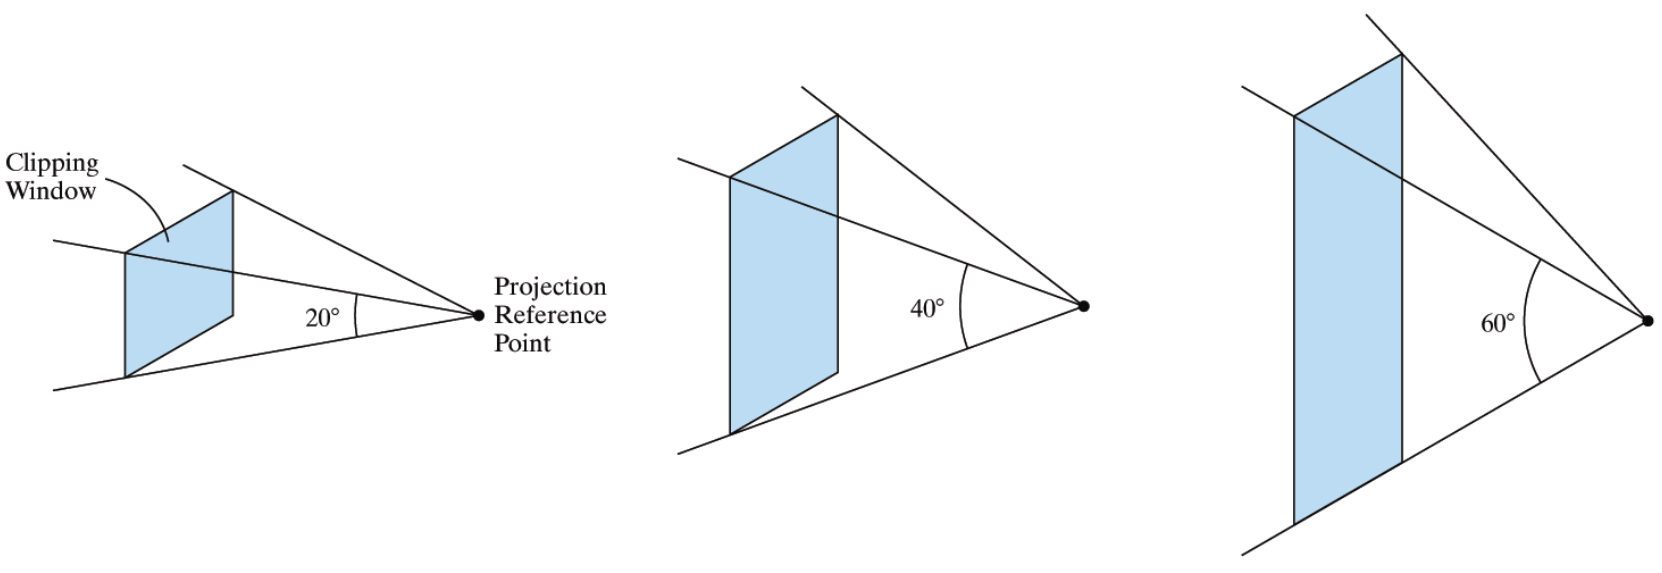
\includegraphics[width=1\textwidth]{Figures/Zoo}
			\end{center}
	\end{figure}
\end{frame}

%%%%%%%%%%%%%%%%%%%%%%%%%%%%%%%%%%%%%%%%%%%%%%%%%%%%%%%%%%%%%%%%%%%%%%%%%%%%%%%%%%%%%%%%%%
\begin{frame}
\frametitle{Transformações de Coordenadas de Projeção Perspectiva}
	\begin{block}{Frustrum Oblíquo}
		\begin{itemize}
			\item Se a linha que parte do centro de projeção  e cruza o centro da janela de recorte  não intersecta a linha central do Frustrum de projeção e perspectiva, então temos um \textbf{Frustrum oblíquo}.
			\begin{itemize}
				\item Então é necessário transformar este Frustrum é um Frustum simétrico.
			\end{itemize}
		\end{itemize}	
	\end{block}
	
		\begin{figure}[!h]
			\begin{center}
			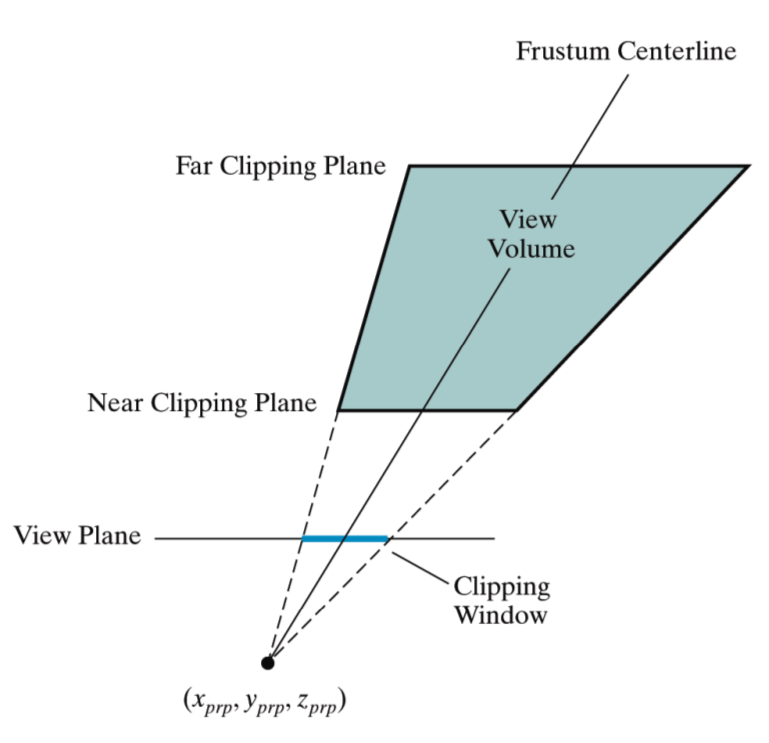
\includegraphics[width=0.4\textwidth]{Figures/FruObl}
			\end{center}
	\end{figure}
\end{frame}


%%%%%%%%%%%%%%%%%%%%%%%%%%%%%%%%%%%%%%%%%%%%%%%%%%%%%%%%%%%%%%%%%%%%%%%%%%%%%%%%%%%%%%%%%%
\begin{frame}
\frametitle{Transformações de Coordenadas de Projeção Perspectiva}
	\begin{block}{Frustrum Oblíquo}
		\begin{itemize}
			\item Esta transformação pode ser obtida fazendo o cisalhamento em z.
		\end{itemize}	
	\end{block}
	
		\begin{figure}[!h]
			\begin{center}
			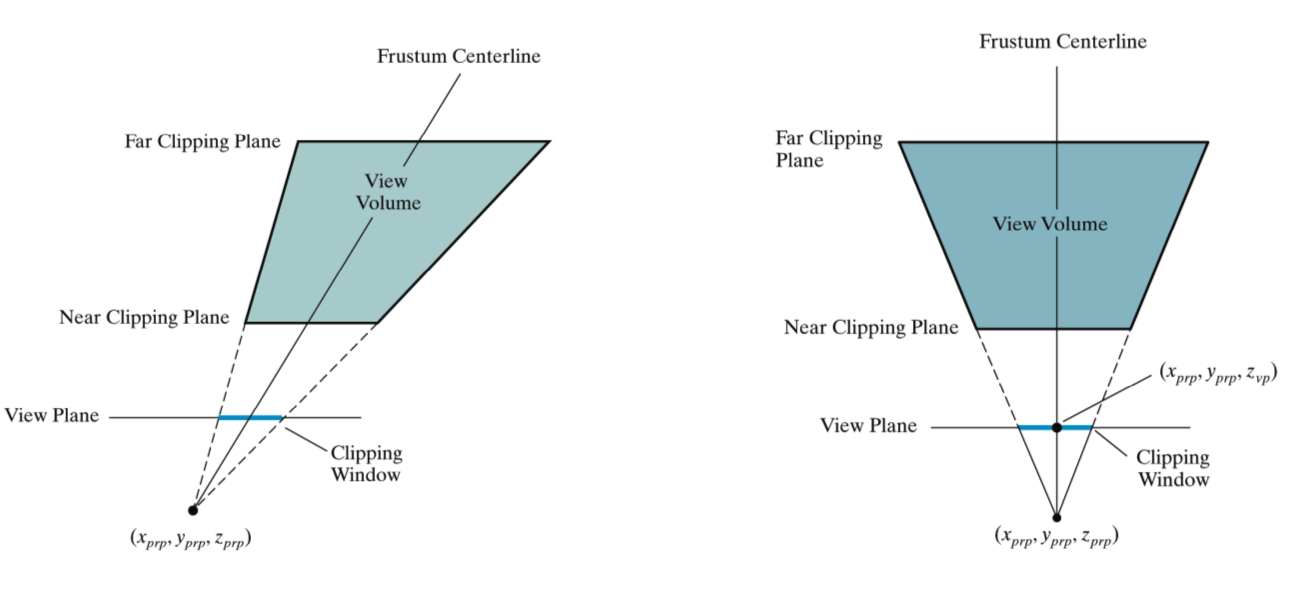
\includegraphics[width=0.9\textwidth]{Figures/TraFru}
			\end{center}
	\end{figure}
\end{frame}

%%%%%%%%%%%%%%%%%%%%%%%%%%%%%%%%%%%%%%%%%%%%%%%%%%%%%%%%%%%%%%%%%%%%%%%%%%%%%%%%%%%%%%%%%%
\begin{frame}
\frametitle{Transformações de Coordenadas de Projeção Perspectiva}
	\begin{block}{Normalização}
		\begin{itemize}
			\item O ultimo passo da projeção perspectiva é mapear o paralelepípedo para um \textbf{volume normalizado}.
		\end{itemize}	
	\end{block}
	
		\begin{figure}[!h]
			\begin{center}
			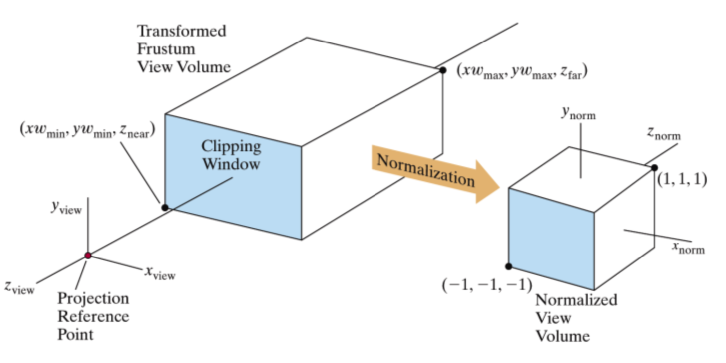
\includegraphics[width=0.9\textwidth]{Figures/VolVisNor}
			\end{center}
	\end{figure}
\end{frame}

%%%%%%%%%%%%%%%%%%%%%%%%%%%%%%%%%%%%%%%%%%%%%%%%%%%%%%%%%%%%%%%%%%%%%%%%%%%%%%%%%%%%%%%%%%
\section{Algoritmos de Recorte 3D}

\begin{frame}
\frametitle{Algoritmos de Recorte 3D}
	\begin{block}{Algoritmos de Recorte 3D}
		\begin{itemize}
			\item Com o cubo normalizado os algoritmos de recorte podem ser aplicados com maior eficiência.
			\item Os algoritmos de recorte eliminam os objetos fora do volume de visão e processão o resto.
			\item São extensões dos algoritmos de recorte 2D, mas com planos como fronteiras ao invés de linhas.
			\item O recorte é aplicado após todas as transformações serem aplicadas.
		\end{itemize}	
	\end{block}
	
\end{frame}


%%%%%%%%%%%%%%%%%%%%%%%%%%%%%%%%%%%%%%%%%%%%%%%%%%%%%%%%%%%%%%%%%%%%%%%%%%%%%%%%%%%%%%%%%%
\begin{frame}
\frametitle{Algoritmos de Recorte 3D}
	\begin{block}{Algoritmos de Recorte 3D}
		\begin{itemize}
			\item No pipeline 3D temos que os pontos processados utilizando as matrizes de transformações geométricas estão em uma representação homogênea.
			\begin{equation*}
				\begin{bmatrix}
					x_h \\
					y_h \\
					z_h \\
					h
				\end{bmatrix}
				= \textbf{M} \cdot \begin{bmatrix}
					x \\
					y \\
					z \\
					1
				\end{bmatrix}
			\end{equation*}
			\item Onde \textbf{M} é a concatenação de todas as matrizes.
			\item Um método de recorte efetivo é aplicar as rotinas de recorte na representação homogênea.
			\begin{itemize}
				\item Os procedimentos de recorte podem ser iguais em qualquer tipo de projeção aplicada.
			\end{itemize}
		\end{itemize}	
	\end{block}
	
\end{frame}


%%%%%%%%%%%%%%%%%%%%%%%%%%%%%%%%%%%%%%%%%%%%%%%%%%%%%%%%%%%%%%%%%%%%%%%%%%%%%%%%%%%%%%%%%%
\begin{frame}
\frametitle{Algoritmos de Recorte 3D}
	\begin{block}{Código de Região 3D}
		\begin{itemize}
			\item O conceito de código de região 2D (Algoritmo de Cohen-Sutherland) pode ser estendido  para representações 3D adicionando mais alguns bits.
			\begin{itemize}
				\item Código de 6 bits.
			\end{itemize}
		\end{itemize}	
	\end{block}
	
	\begin{figure}[!h]
			\begin{center}
			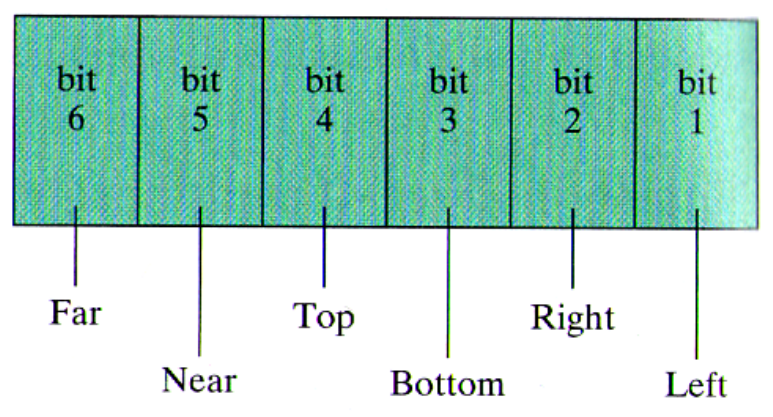
\includegraphics[width=0.6\textwidth]{Figures/CodReg}
			\end{center}
	\end{figure}
\end{frame}

%%%%%%%%%%%%%%%%%%%%%%%%%%%%%%%%%%%%%%%%%%%%%%%%%%%%%%%%%%%%%%%%%%%%%%%%%%%%%%%%%%%%%%%%%%
\begin{frame}
\frametitle{Algoritmos de Recorte 3D}
	\begin{block}{Código de Região 3D}
		\begin{itemize}
			\item Os valores dos bits são calculados de forma semelhante ao 2D.
			\begin{itemize}
				\item 0 está dentro de uma fronteira, 0 está fora.
			\end{itemize}
		\end{itemize}	
	\end{block}
	
	\begin{figure}[!h]
			\begin{center}
			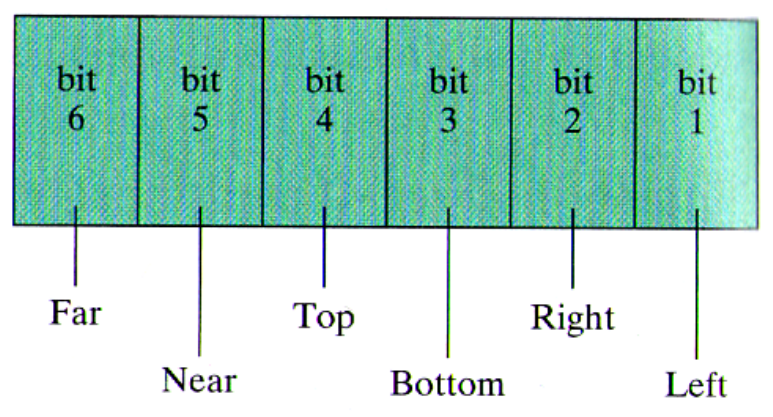
\includegraphics[width=0.6\textwidth]{Figures/CodReg}
			\end{center}
	\end{figure}
\end{frame}

%%%%%%%%%%%%%%%%%%%%%%%%%%%%%%%%%%%%%%%%%%%%%%%%%%%%%%%%%%%%%%%%%%%%%%%%%%%%%%%%%%%%%%%%%%
\begin{frame}
\frametitle{Algoritmos de Recorte 3D}
	\begin{block}{Código de Região 3D}
		\begin{itemize}
			\item Considerando que estamos trabalhando com coordenadas homogêneas $P=(x_h,y_h,z_h,h)$, um ponto dentro do volume de visão deve satisfazer:
			\begin{eqnarray*}
				-1 \leq \frac{x_h}{h} \leq 1 \\
				-1 \leq \frac{y_h}{h} \leq 1 \\
				-1 \leq \frac{z_h}{h} \leq 1 \\
			\end{eqnarray*}
		\end{itemize}	
	\end{block}
\end{frame}

%%%%%%%%%%%%%%%%%%%%%%%%%%%%%%%%%%%%%%%%%%%%%%%%%%%%%%%%%%%%%%%%%%%%%%%%%%%%%%%%%%%%%%%%%%
\begin{frame}
\frametitle{Algoritmos de Recorte 3D}
	\begin{block}{Código de Região 3D}
		\begin{itemize}
			\item Com $P=(x_h,y_h,z_h,h)$ e assumindo $h \neq 0$ podemos calcular:
			\begin{itemize}
				\item se $h > 0$
					\begin{eqnarray*}
					-h \leq x_h \leq h \\
					-h \leq y_h \leq h \\
					-h \leq z_h \leq h \\
					\end{eqnarray*}
				\item se $h < 0$
					\begin{eqnarray*}
						h \leq x_h \leq -h \\
						h \leq y_h \leq -h \\
						h \leq z_h \leq -h \\
					\end{eqnarray*}
			\end{itemize}
			
		\end{itemize}	
	\end{block}
\end{frame}

%%%%%%%%%%%%%%%%%%%%%%%%%%%%%%%%%%%%%%%%%%%%%%%%%%%%%%%%%%%%%%%%%%%%%%%%%%%%%%%%%%%%%%%%%%
\begin{frame}
\frametitle{Algoritmos de Recorte 3D}
	\begin{block}{Código de Região 3D}
		\begin{itemize}
			\item Com $h>0$ podemos definir os valores dos bits como:
			\begin{eqnarray*}
				bit_1 = 1 \: se \: h + x_h < 0 \:(esquerda)
			\end{eqnarray*}
		\end{itemize}	
	\end{block}
\end{frame}

%%%%%%%%%%%%%%%%%%%%%%%%%%%%%%%%%%%%%%%%%%%%%%%%%%%%%%%%%%%%%%%%%%%%%%%%%%%%%%%%%%%%%%%%%%
\begin{frame}
\frametitle{Algoritmos de Recorte 3D}
	\begin{figure}[!h]
			\begin{center}
			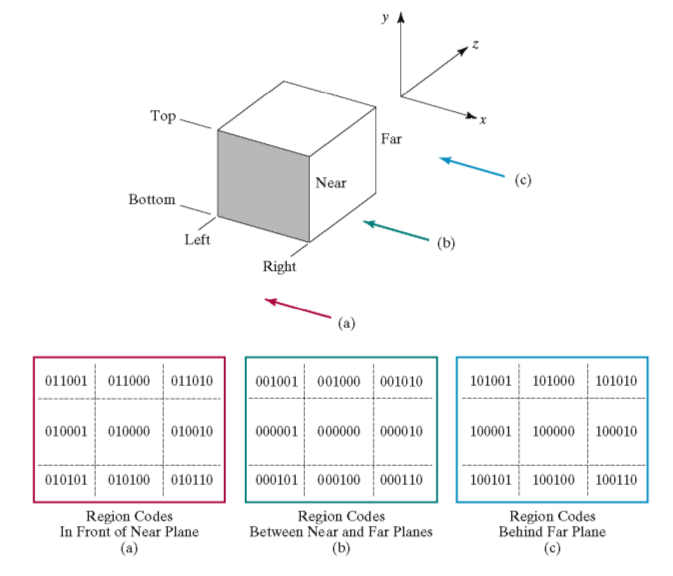
\includegraphics[width=0.8\textwidth]{Figures/CodCoo}
			\end{center}
	\end{figure}
\end{frame}

%%%%%%%%%%%%%%%%%%%%%%%%%%%%%%%%%%%%%%%%%%%%%%%%%%%%%%%%%%%%%%%%%%%%%%%%%%%%%%%%%%%%%%%%%%
\begin{frame}
\frametitle{Algoritmos de Recorte 3D}
	\begin{block}{Recorte de Linhas}
		\begin{itemize}
			\item O recorte de linha é essencialmente o mesmo que o recorte de linha 2D.
			\begin{itemize}
				\item Se ambos os pontos finais da linhas são 000000, a linha está dentro.
				\item Uma linha está dentro se a operação ``\textbf{ou}'' sobre seus pontos finais for igual a 000000.
				\item Uma linha está fora se a operação ``e'' sobre seus pontos finais for diferente de 000000. 
			\end{itemize}			 
		\end{itemize}	
	\end{block}
\end{frame}

%%%%%%%%%%%%%%%%%%%%%%%%%%%%%%%%%%%%%%%%%%%%%%%%%%%%%%%%%%%%%%%%%%%%%%%%%%%%%%%%%%%%%%%%%%
\begin{frame}
\frametitle{Algoritmos de Recorte 3D}
	\begin{figure}[!h]
			\begin{center}
			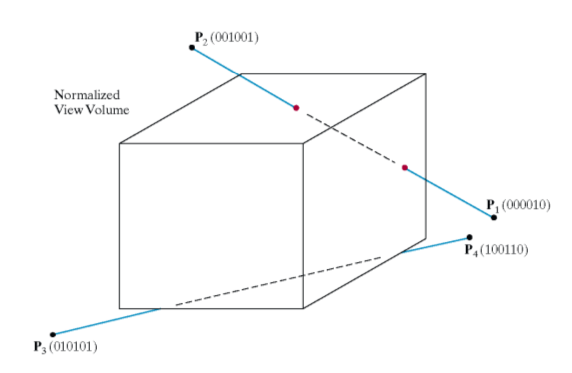
\includegraphics[width=0.8\textwidth]{Figures/RecLin}
			\end{center}
	\end{figure}
\end{frame}

%%%%%%%%%%%%%%%%%%%%%%%%%%%%%%%%%%%%%%%%%%%%%%%%%%%%%%%%%%%%%%%%%%%%%%%%%%%%%%%%%%%%%%%%%%
\begin{frame}
\frametitle{Algoritmos de Recorte 3D}
	\begin{block}{Recorte de Polígonos 3D}
		\begin{itemize}
			\item Pacotes gráficos geralmente lidam com os objetos descritos com equações lineares, sendo assim, as intersecções das arestas dos objetos com o plano de recorte são utilizadas para delimitar o objeto.
			\item Além disso, algumas rotinas simples como o \textbf{bounding box} podem ser utilizadas para definir se um polígono está dentro ou fora das fronteiras.			 
		\end{itemize}	
	\end{block}
\end{frame}

%----------------------------------------------------------------------------------------
\end{document} 